%!TEX root=./LIVRO.tex
\captionsetup{font={small, it}}
\captionsetup{justification=raggedright, singlelinecheck=false}

\chapter{Apresentação da plataforma}

% Odoo em Portugal, características técnicas (eLeading, Survey)
\lipsum[1]

Nonnono\footnote{Citar em nota o Odoo.}


\begin{figure}[t]
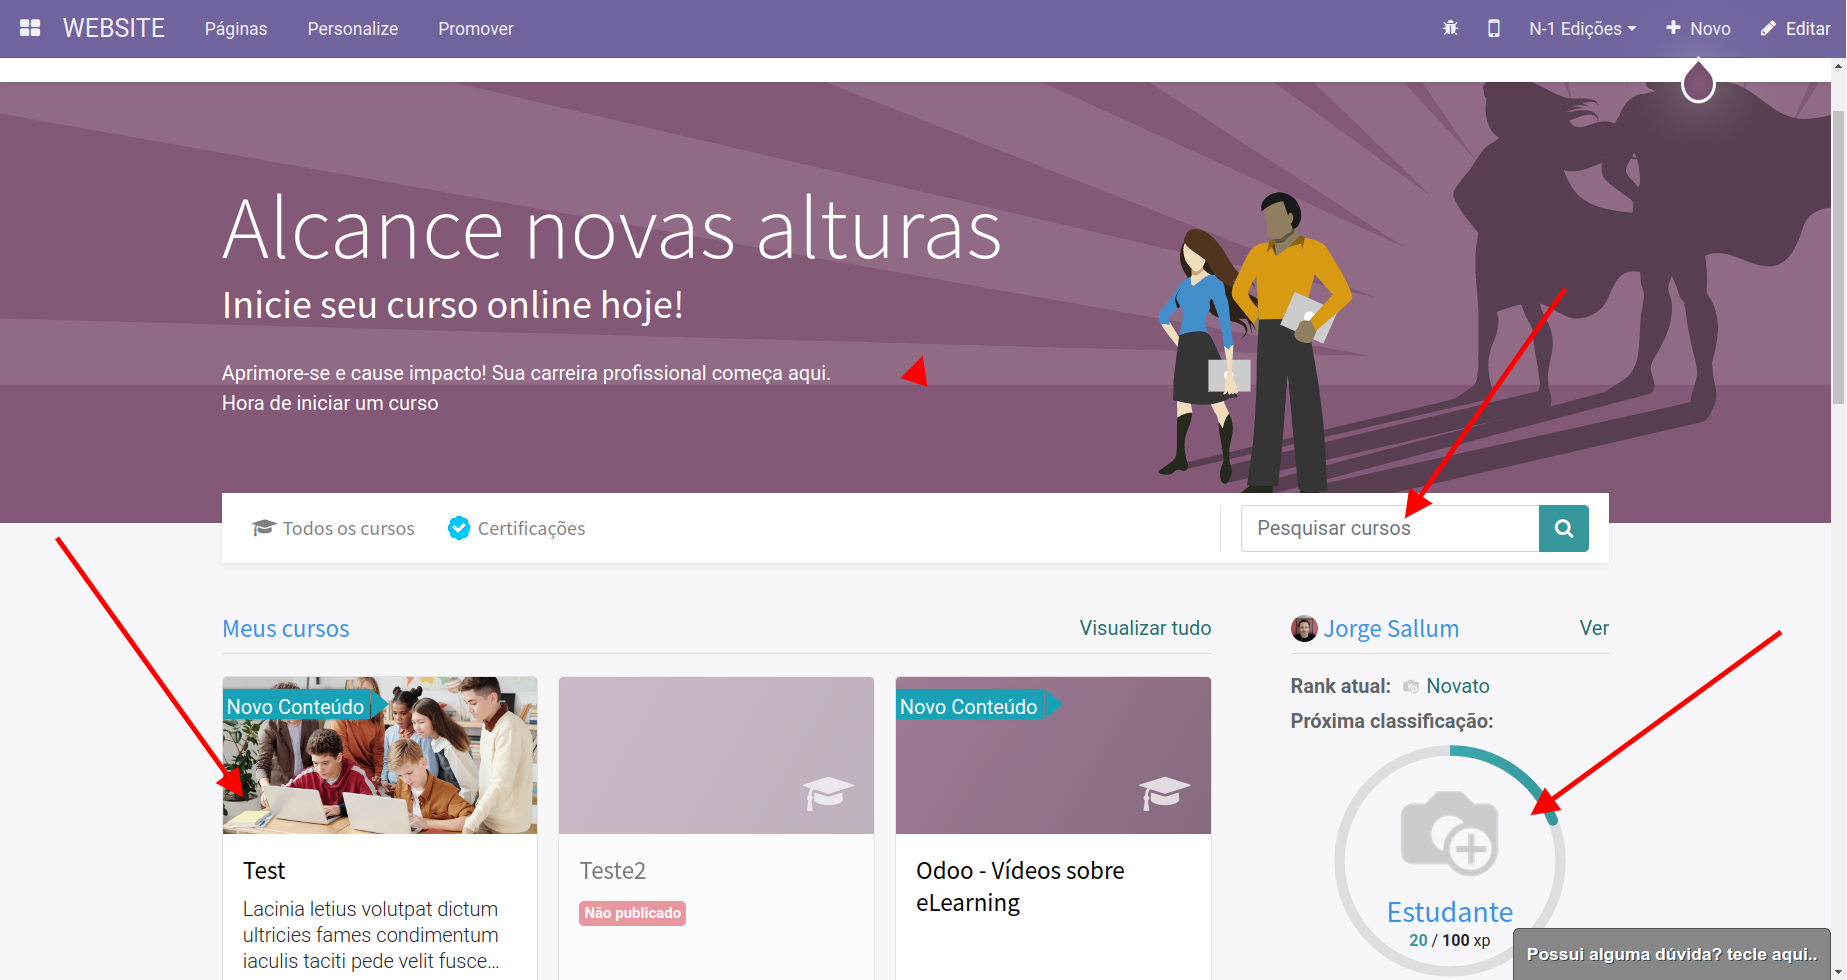
\includegraphics[width=\textwidth]{imgs/screenshot1}
\end{figure}


\section{A quem se destina}
% Felipe

\lipsum[1-3]
% Quantos cursos, como estão dividas as seções, natureza dos conteúdo

\section{Como acessar?}

% Jorge

\lipsum[1-3]
\begin{figure}[t]
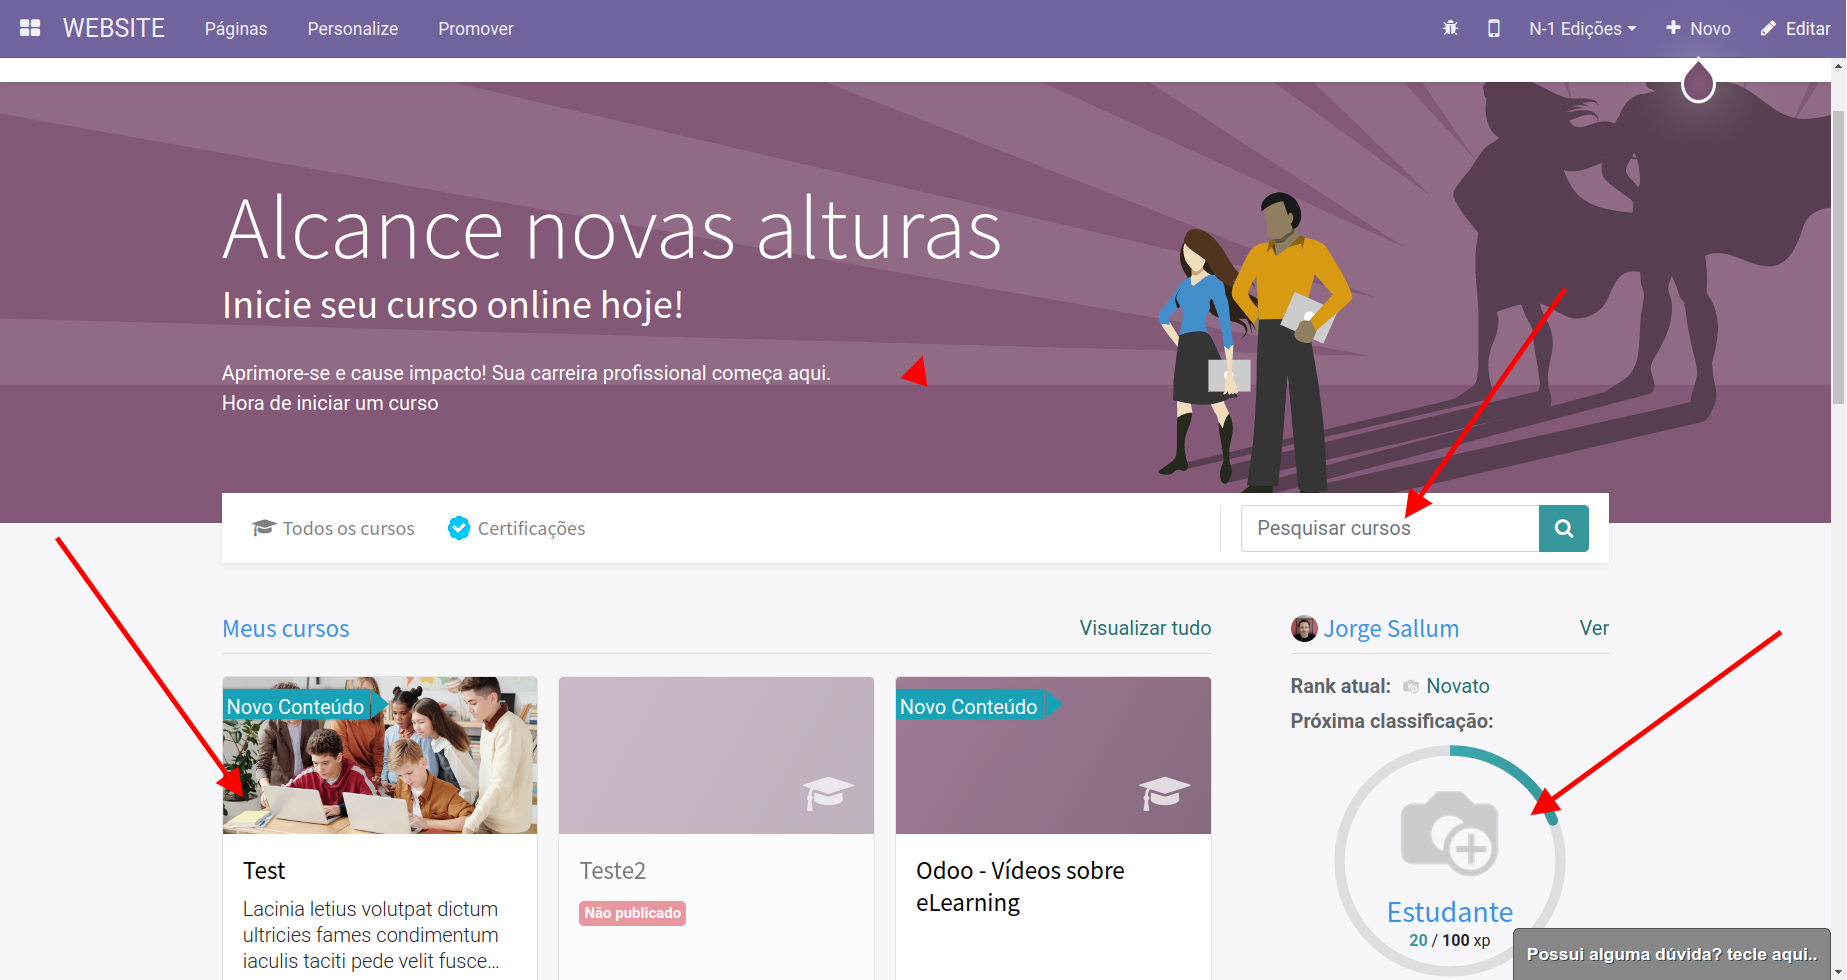
\includegraphics[width=\textwidth]{imgs/screenshot2}
\end{figure}

\section{Apresentação do conteúdo digital}

% André
% Explicar as seções, a relação com o material impresso, os quiz

\lipsum[1-3]

\section{Estrutura do site} % Jorge




